\documentclass[12pt, a4paper]{article} 
% --- MARGINS ---
\usepackage[margin=2.5cm]{geometry} 
% --- PACKAGES ---
\usepackage{graphicx}
\usepackage{textcomp}
\usepackage[hungarian]{babel}
\usepackage[T1]{fontenc}
\usepackage[utf8]{inputenc}
\usepackage{caption}
\usepackage{subcaption}
\usepackage{csquotes}
\usepackage{siunitx}

% --- IMAGES PATH ---
\graphicspath{{./Pictures/}{./Pictures/koax}{./Pictures/erosito}{./Pictures/Kisjelu-erositok}{./Pictures/Nagyjelu-erositok}{./Pictures/Keverok-es-oszcillatorok}{./Pictures/Forrasztos}}

% --- BIBLIOGRAPHY ---
\usepackage[style=ieee]{biblatex}
\addbibresource{forrasok.bib}

% --- CODE LISTINGS ---
\usepackage{listings}
\usepackage[dvipsnames]{xcolor}
\usepackage{amsmath}
\usepackage{placeins}

% --- COLORS & SETTINGS ---
\definecolor{dkgreen}{rgb}{0,0.6,0}
\definecolor{gray}{rgb}{0.5,0.5,0.5}
\definecolor{mauve}{rgb}{0.58,0,0.82}

\lstset{frame=tb,
  language=Bash,
  aboveskip=3mm,
  belowskip=3mm,
  showstringspaces=false,
  columns=flexible,
  basicstyle={\small\ttfamily},
  numbers=none,
  numberstyle=\tiny\color{gray},
  keywordstyle=\color{blue},
  commentstyle=\color{dkgreen},
  stringstyle=\color{mauve},
  breaklines=true,
  breakatwhitespace=true,
  tabsize=2
}

\title{Yagi antenna szimulációja}
\author{Nyiri Levente}
\date{2026 Január}

\begin{document}

\begin{titlepage}
    \centering
    \includegraphics[width=\textwidth]{BME.png}\par\vspace{1cm}
    
    {\huge\bfseries Yagi antenna szimulációja \par}
    \vspace{1.5cm}
    {\Large\itshape Nyiri Levente \par}
    \vspace{1cm}
    {\large 2026. január \par}
    
    \vfill
    % Itt maradhat üresen, vagy ide jöhet egyéb infó (pl. konzulens)
\end{titlepage}

\tableofcontents

\selectlanguage{hungarian}

\newpage

\section{Bevezetés}

A Yagi-Uda antennát Shintaro Uda és Hidetsuru Yagi találta fel az 1920-as években. Uda Yagi asszisztense volt, eredetileg eredményeiket japánul dokumentálta, így a világ többi részén csak akkor lett ismert, amikor Yagi  leírta azokat angolul is. Annak ellenére, hogy kreditálta Uda munkáját, az antennára leggyakrabban csak Yagi antennaként hivatkoznak.

Ez egy antennarendszer, amelyben egy dipólantennát vesznek körül parazita elemekkel, hogy jobb irányítottságot érjenek el.

Az elmúlt évtizedekben ez lett a legelterjedtebb antenna TV vételére VHF és UHF sávokon.

A feladatomhoz kaptam  egy dokumentumot, amelyben különböző Yagi antenna dimenziók vannak megadva VHF sávon, ebből fogok kiindulni, egy 58 MHz-es antennát fogok tervezni a K 52 16 8 27-es oszlop alapján.

\begin{figure}[ht]
    \centering
    \includegraphics[width=0.8\textwidth]{kathrein.jpg} 
    \caption{Antenna dimenziók}
    \label{fig:kathrein}
\end{figure}



\clearpage

\section{Elméleti ismeretek összefoglalása}

Egy Yagi antenna 3 részből áll: egy reflektorból (ritkán alkalmaznak többet, mivel jelentősen nem javítja az irányítottságot az elemszám növelése, jelen esetben 3 elemből áll), egy táplált félhullámú dipólból (a továbbiakban DE, mint driven element-ként fogok rá hivatkozni) és egy vagy több direktorból.
A felépítést a \ref{fig:yagi-konyv}. ábra mutatja. A DE leggyakrabban egy hajlított dipólus, én a szimulációban egyszerű vezetéket alkalmaztam.


\begin{figure}[ht]
    \centering
    \includegraphics[width=0.6\textwidth]{Yagi-konyv.png} 
    \caption{Yagi antenna általános felépítése \cite{balanis}}
    \label{fig:yagi-konyv}
\end{figure}

A reflektor valamivel nagyobb, mint a DE, a direktorok pedig valamivel kisebbek.

A sugárzási irány a direktorok irányába mutat, és minél több direktort használunk, annál jobb az irányító hatás, bár egy bizonyos szám fölött már elhanyagolható a javulás, inkább több Yagi antenna egymás mellé rakásával szoktak függönyantennát létrehozni.

Mivel a reflektor hosszabb mint a DE, ezért az impedanciája induktív lesz, a direktoroké (mivel ők pedig rövidebbek) kapacitív. Ez egy fázisprogresszióhoz fog vezetni az antenna mentén, amely hasonló lesz egy haladóhulláméhoz, a DE terét a direktorok irányába fogja erősíteni. 

A Yagi antennarendszerre tekinthetünk egy olyan struktúraként, amely egy haladóhullámot támogat, amelynek a teljesítménye az egyes elemek árameloszlásán és a fázissebességen múlik \cite{balanis}.

\clearpage

\section{Tervezés}

A tervezés során a célom, hogy eredményképpen egy olyan antennát kapjak, amely tükrözi a(z) \ref{fig:kathrein}. ábrát, tehát:

\begin{itemize}
    \item \textbf{VSWR:} $< 1.15$.
    \item \textbf{Gain:} Legalább 6 dBi.
    \item \textbf{Bemeneti impedancia:} 50 $\Omega$.
    \item \textbf{Iránykarakterisztika:} A \ref{fig:kathrein}. ábrához hasonló.
\end{itemize}

Az adott értékek:
\begin{table}[ht]
    \centering
    \begin{tabular}{|clc|}
        \hline
        \textbf{Szimbólum} & \textbf{Leírás} & \textbf{Érték[m]} \\ \hline
        A & Reflektor és utolsó direktor távolsága & 2.95 \\
        B & Reflektor hossza & 2.51 \\
        C & Reflektorok távolsága Z síkban & 1.95 \\ \hline
    \end{tabular}
    \caption{Az adott dimenziók}
    \label{tab:dimenziok}
\end{table}

A szimulációt szabadtérben végeztem, a vezető anyagának rezet adtam meg, a kábelek sugarát 0.0025$\lambda$-nak választottam.

Parazitikus elemek jelenlétében a DE optimális hossza nem pontosan 0.5$\lambda$, hanem valahol 0.45-0.49$\lambda$ között van \cite{balanis}.

Bár az "Antenna Theory Analysis and Design" könyv azt írja, hogy tipikusan a direktorok közt 0.3-0.4$\lambda$ hely van, ez jelen esetben nem megvalósítható, mivel a reflektor és az utolsó direktor közti távolság adott, és túl nagy lenne a lépésköz. Más forrásokban azt találtam, hogy 0.25-0.05$\lambda$ közti távolságokat gyakran alkalmaznak \cite{yagi-video}.

Az optimális tervhez a direktorok közti távolság nem konstans. Kiindulásképpen beállítottam ezeket a távolságokat megfelelő kompromisszumnak tűnő értékekre.


A Chen és Cheng által publikált optimalizálási eljárását látva \cite{cheng}, illetve figyelembe véve, hogy a front-to-back ratio milyen érzékeny a direktorok távolságára (lásd \ref{fig:dir-spacing-balanis}. ábra), a 4nec2 optimizer használatával finomhangoltam ezeket a paramétereket.
\begin{figure}[ht]
    \centering
    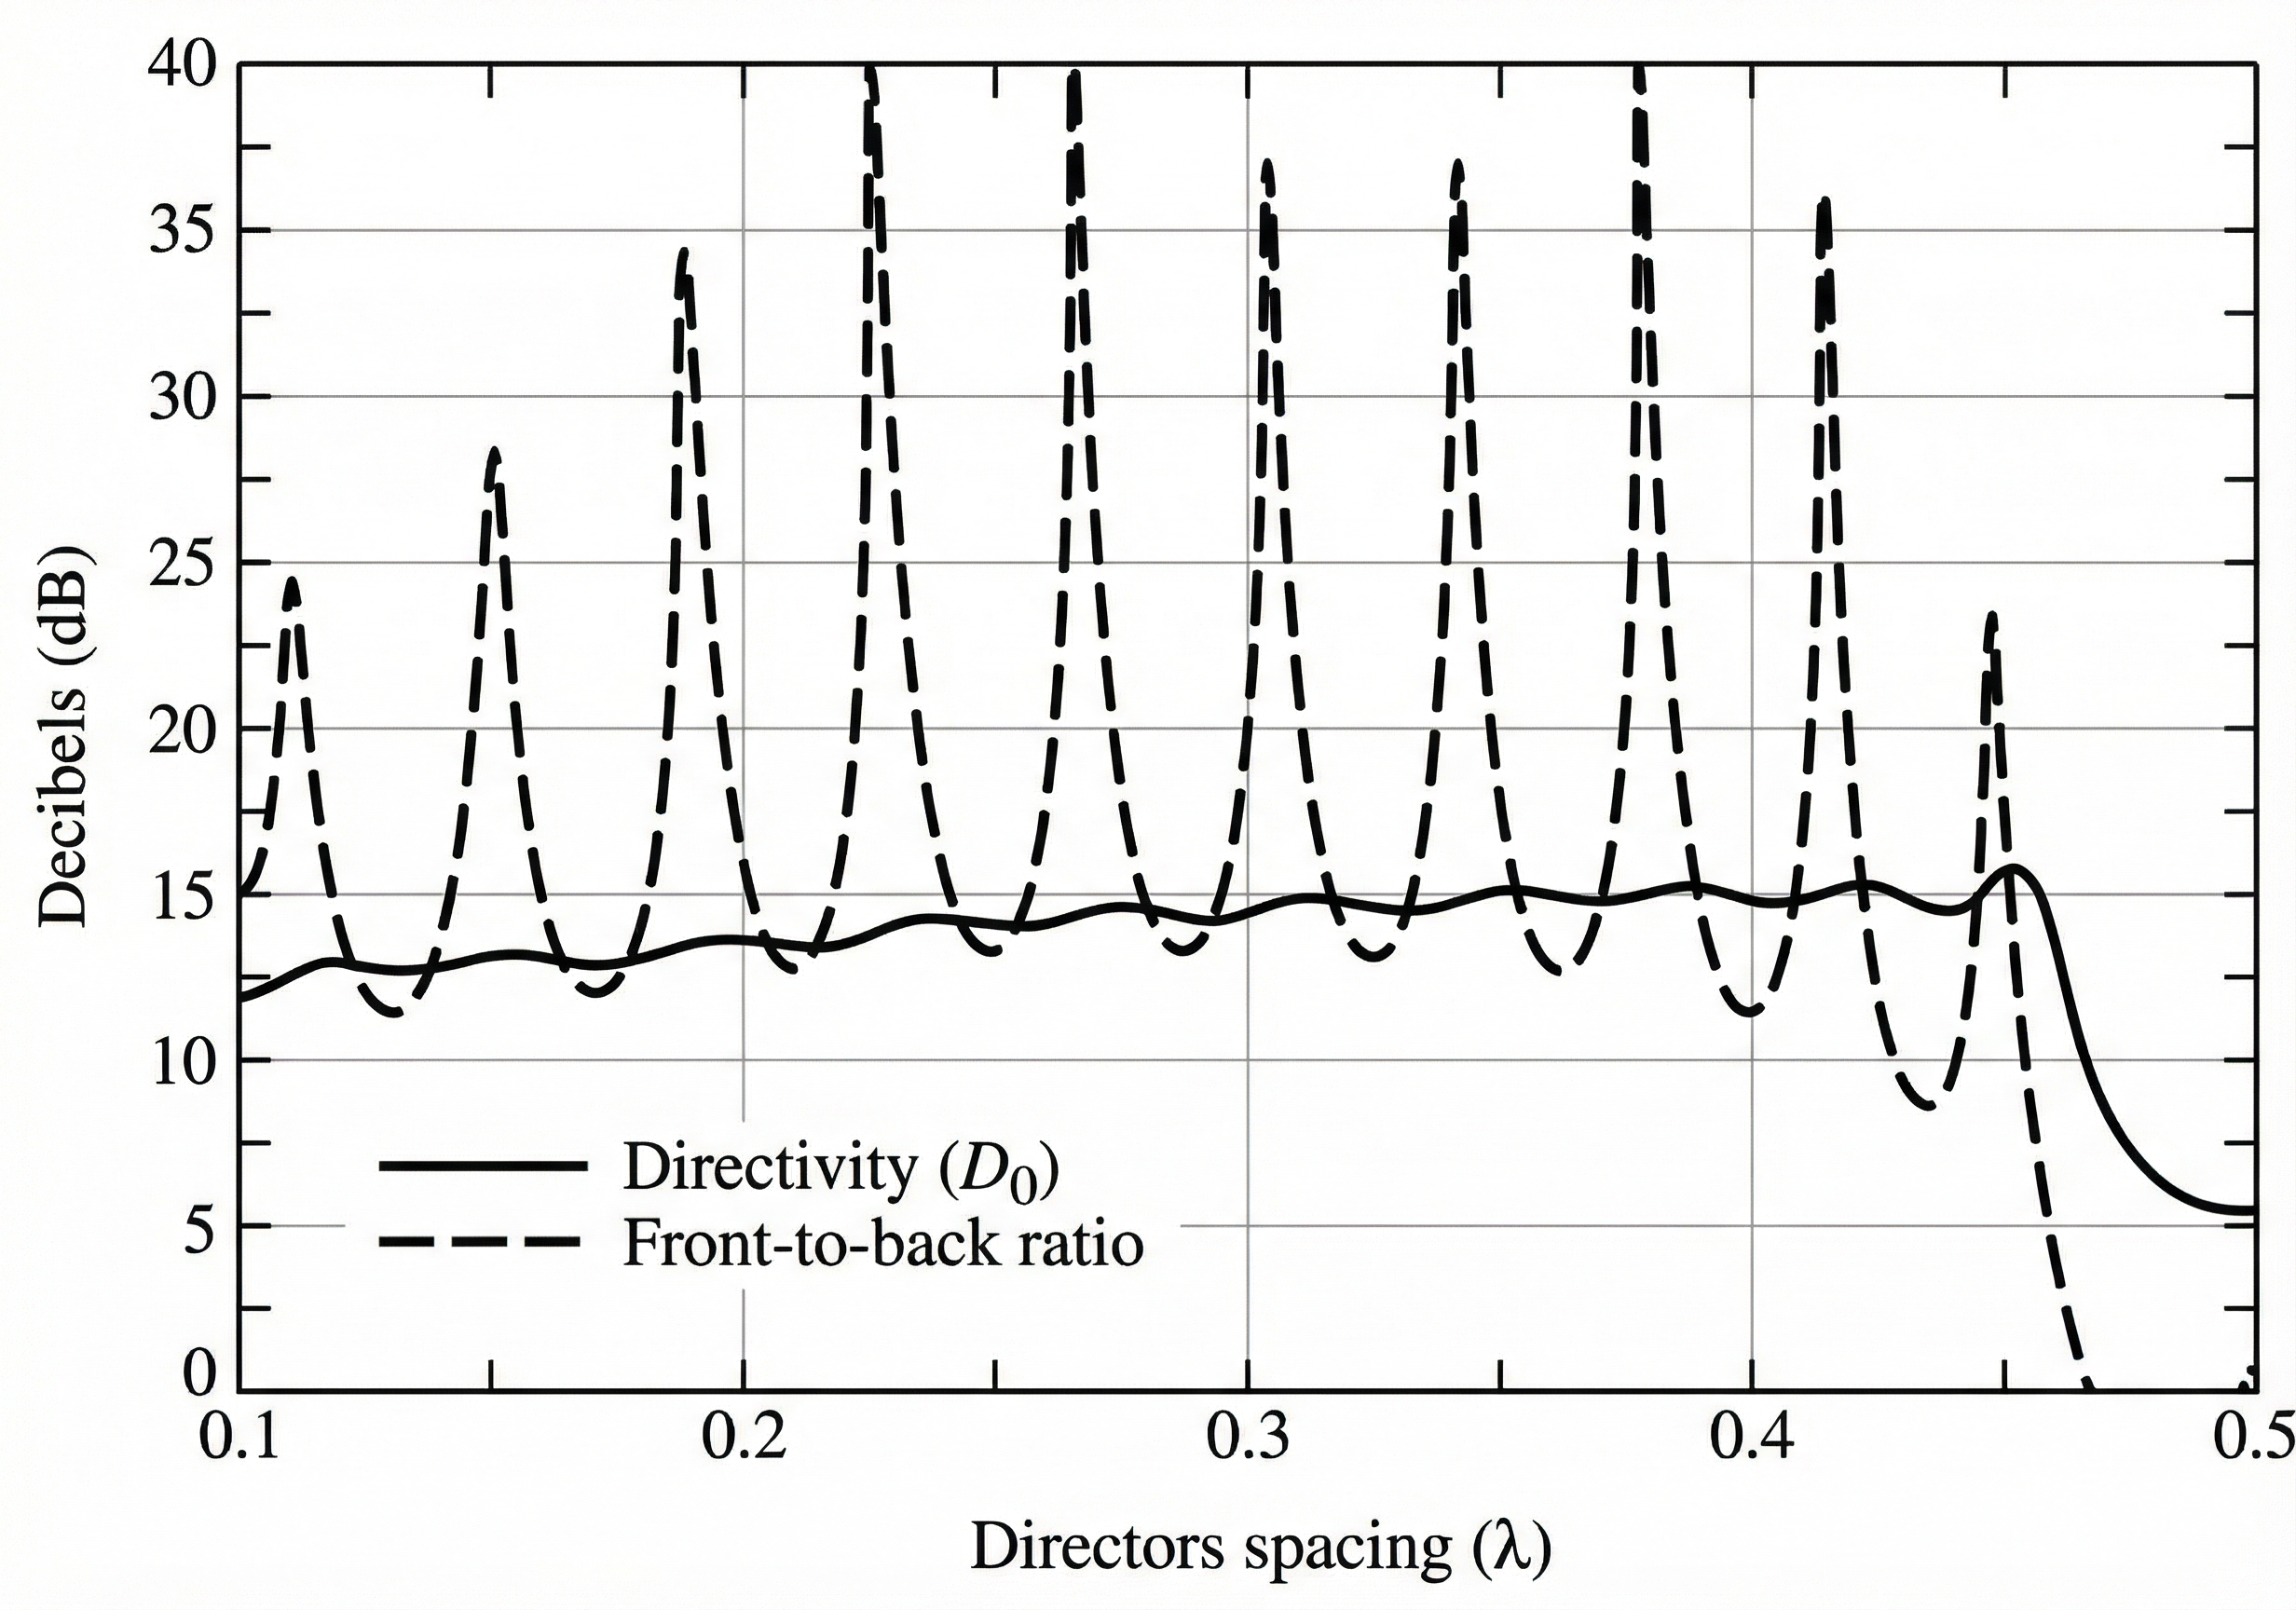
\includegraphics[width=0.7\textwidth]{dir-spacing-balanis.png} 
    \caption{Front-to-back ratio érzékenysége a direktorok távolságaira \cite{balanis}}
    \label{fig:dir-spacing-balanis}
\end{figure}
Először csak az SWR-re és a reaktanciára egyenlő súllyal futtattam csak a direktorok távolságára. A következő futtatásnál megadtam paraméternek a DE és a direktor hosszát is, a DE és a reflektor távolságát, és a DE-direktor illetve a direktorok távolságát. Ezúttal előre-hátra viszonyra, SWR-re és reaktanciára egyenlő súlyokkal optimalizáltam.

Az eredeti és az optimalizált értékeket a \ref{tab:yagi_parameters}. táblázat mutatja.

\begin{table}[ht]
    \centering
    \begin{tabular}{|lcc|}
        \hline
        \textbf{Paraméter} & \textbf{Eredeti érték} & \textbf{Optimalizált érték} \\ \hline
        Sugárzó hossza (DE) & 0.48$\lambda$ & 0.48$\lambda$ \\
        Direktorok hossza & 0.45$\lambda$ & 0.45$\lambda$ \\ 
        Reflektor--DE távolság & 0.15$\lambda$ & 0.2$\lambda$ \\ 
        Sugárzó--D1 távolság & 0.15$\lambda$ & 0.15$\lambda$ \\ 
        D1--D2 távolság & 0.1$\lambda$ & 0.083$\lambda$ \\ 
        D2--D3 távolság & 0.08$\lambda$ & 0.054$\lambda$ \\ 
        D3--D4 távolság & 0.06$\lambda$ & 0.062$\lambda$ \\ \hline
    \end{tabular}
    \caption{A Yagi antenna eredeti és optimalizált paraméterei}
    \label{tab:yagi_parameters}
\end{table}

\FloatBarrier

Optimalizálás előtt a VSWR 4.45 volt, utána 1.14, tehát jelentősen javult a geometriának az enyhe módosításával, anélkül, hogy a nyereséget negatívan befolyásolta volna. Az is látszik, hogy a DE és a direktorok hossza nem változott (illetve csak olyan csekély mértékben, hogy $\lambda$-ban kifejezve elhanyagolható).

\begin{figure}[ht]
     \centering
     \begin{subfigure}[b]{0.48\textwidth}
         \centering
         \includegraphics[width=\textwidth]{main-58-pre-opt.png}
         \caption{Eredeti adatokkal mért eredmények}
         \label{fig:main-pre}
     \end{subfigure}
     \hfill 
     \begin{subfigure}[b]{0.48\textwidth}
         \centering
         \includegraphics[width=\textwidth]{main-58.png}
         \caption{Optimalizált adatokkal mért eredmények}
         \label{fig:main}
     \end{subfigure}
     
     \caption{Eredeti és optimalizált állapot}
     \label{fig:osszehasonlitas}
\end{figure}

A reflektor és a DE távolsága főként az előre-hátra viszonyra és a bemeneti impedanciára van hatással \cite{balanis}, szóval kíváncsiságból minden mást változatlanul hagyva megváltoztattam a reflektor-DE távolságot 0.2$\lambda$-ra, és már így is 2.4-re javult a VSWR. 

A következő ábrákon a frekvencia függvényében látható az SWR (\ref{fig:SWR}. ábra), a nyereség, front-to-back és front-to-rear ratio (\ref{fig:GAIN}. ábra), valamint az impedancia (\ref{fig:IMP}.ábra) .

A \ref{fig:irany}. ábrán látható az iránykarakterisztika.

Az utánuk következő ábrákon pedig az antenna 3D modellje, az egyes szegmenseken folyó áramok nagysága és fázisa (\ref{fig:HE}. ábra), valamint a távoltér 3D reprezentációja látható (\ref{fig:TAVOLTER}. ábra).
\begin{figure}[ht]
     \centering
     \begin{subfigure}[b]{0.48\textwidth}
         \centering
         \includegraphics[width=\textwidth]{SWR-58-pre-opt.png}
         \caption{Eredeti}
         \label{fig:swr-pre}
     \end{subfigure}
     \hfill 
     \begin{subfigure}[b]{0.48\textwidth}
         \centering
         \includegraphics[width=\textwidth]{SWR-58.png}
         \caption{Optimalizált}
         \label{fig:swr}
     \end{subfigure}
     
     \caption{Eredeti és optimalizált \textcolor{blue}{SWR} és \textcolor{red}{reflexiós} tényező frekvencia függvényében}
     \label{fig:SWR}
\end{figure}


\begin{figure}[ht]
     \centering
     \begin{subfigure}[b]{0.48\textwidth}
         \centering
         \includegraphics[width=\textwidth]{gain-58-pre-opt.png}
         \caption{Eredeti}
         \label{fig:gain-pre}
     \end{subfigure}
     \hfill 
     \begin{subfigure}[b]{0.48\textwidth}
         \centering
         \includegraphics[width=\textwidth]{gain-58.png}
         \caption{Optimalizált}
         \label{fig:gain}
     \end{subfigure}
     
     \caption{Eredeti és optimalizált \textcolor{blue}{nyereség} és \textcolor{red}{F/B} valamint \textcolor{ForestGreen}{F/R}}
     \label{fig:GAIN}
\end{figure}

\begin{figure}[ht]
     \centering
     \begin{subfigure}[b]{0.48\textwidth}
         \centering
         \includegraphics[width=\textwidth]{imp-58-pre-opt.png}
         \caption{Eredeti}
         \label{fig:imp-pre}
     \end{subfigure}
     \hfill 
     \begin{subfigure}[b]{0.48\textwidth}
         \centering
         \includegraphics[width=\textwidth]{imp-58.png}
         \caption{Optimalizált}
         \label{fig:imp}
     \end{subfigure}
     
     \caption{Eredeti és optimalizált \textcolor{blue}{ellenállás}, \textcolor{red}{reaktancia}, \textcolor{ForestGreen}{impedancia} és \textcolor{magenta}{fázis}}
     \label{fig:IMP}
\end{figure}


\begin{figure}[ht]
     \centering
     \begin{subfigure}[b]{0.48\textwidth}
         \centering
         \includegraphics[width=\textwidth]{H-E-58-pre-opt.png}
         \caption{Eredeti}
         \label{fig:H-E-pre}
     \end{subfigure}
     \hfill 
     \begin{subfigure}[b]{0.48\textwidth}
         \centering
         \includegraphics[width=\textwidth]{H-E-58.png}
         \caption{Optimalizált}
         \label{fig:he}
     \end{subfigure}
     
     \caption{Eredeti és optimalizált iránykarakterisztika}
     \label{fig:irany}
\end{figure}

\begin{figure}[ht]
     \centering
     \begin{subfigure}[b]{0.48\textwidth}
         \centering
         \includegraphics[width=\textwidth]{3D-58.png}
         \caption{3D modell}
         \label{fig:3D}
     \end{subfigure}
     \hfill 
     \begin{subfigure}[b]{0.465\textwidth}
         \centering
         \includegraphics[width=\textwidth]{fazis-aram-58.png}
         \caption{Áram nagysága és fázisa}
         \label{fig:fazis-aram}
     \end{subfigure}
     
     \caption{3D modell és a szegmenseken folyó áramok}
     \label{fig:HE}
\end{figure}

\begin{figure}[ht]
     \centering
     \begin{subfigure}[b]{0.48\textwidth}
         \centering
         \includegraphics[width=\textwidth]{color-58-1-pre-opt.png}
         \caption{Eredeti}
         \label{fig:tavolter-pre}
     \end{subfigure}
     \hfill 
     \begin{subfigure}[b]{0.48\textwidth}
         \centering
         \includegraphics[width=\textwidth]{color-58-1.png}
         \caption{Optimalizált}
         \label{fig:tavolter}
     \end{subfigure}
     
     \caption{Távoltér 3D szimulációja}
     \label{fig:TAVOLTER}
\end{figure}

\FloatBarrier

\subsection*{Eredmények értékelése}
Az \ref{fig:GAIN}. és \ref{fig:irany}. ábrán látszik, hogy az optimalizálás során romlott az előre-hátra viszony, 15.5dB-ről 9.17dB lett. Ez sajnos egy kompromisszum amit el kell fogadnunk az SWR javulásáért cserébe.

A \ref{fig:fazis-aram}. ábrán jól látszik, hogy a reflektoron $\sim \ang{-120}$ a fázis, az első direktoron pedig $\sim \ang{+120}$, tehát a reflektornak induktív, a direktornak kapacitív az impedanciája.

A célkitűzés az volt, hogy a VSWR legyen kisebb mint 1.15, a Gain nagyobb mint 6dBi, bemeneti impedancia 50$\Omega$ és az \ref{fig:kathrein}. ábrához hasonló legyen az iránykarakterisztika.

A kitűzött és az elért értékeket a következő táblázat mutatja.

\begin{table}[ht]
    \centering
    \begin{tabular}{|lcc|}
        \hline
        \textbf{Paraméter} & \textbf{Kitűzött érték} & \textbf{Elért érték} \\ \hline
        VSWR & <1.15 & 1.14 \\
        Gain & >6dBi & 9.47dBi \\
        Bemeneti impedancia & 50$\Omega$ & 43.89$\Omega$ \\ 
        $\Theta_E$ & $\ang{68}$ & $\ang{62}$ \\
        $\Theta_H$ & $\ang{128}$ & $\ang{50}$ \\ \hline 
    \end{tabular}
    \caption{Eredmények}
    \label{tab:eredmeny}
\end{table}

A nyereség és a VSWR kiváló lett, a főnyalábszélességekkel is elégedett vagyok (hacsak nem kifejezetten cél, hogy H síkban nagyobb legyen), az előre-hátra viszony nem éri el a várt értéket.

\clearpage

\section{Összefoglalás}

A projekt során egy 58~MHz-es Yagi-Uda antenna tervezését és szimulációját végeztem el a 4nec2 szoftver segítségével. A tervezési folyamat során egy gyári specifikáció (Kathrein) adataiból indultam ki. 

Először irodalomkutatást végeztem, olvastam az "Antenna Theory Analysis and Design 3rd edition" c. könyv releváns szekcióit és egyéb online  elérhető forrásokat a Yagi-Uda antenna tervezéséről. Utánanéztem a feltalálásának a történelmének is. 

Mikor úgy éreztem, hogy megfelelően utánajártam, elkészítettem 4nec2-ben egy kezdeti geometriát, majd ezt a beépített lehetőségek segítségével optimalizáltam.

Összességében elégedett vagyok az eredményekkel, az előre-hátra viszonytól eltekintve, ami egy 8 elemes Yagi antennához képest jelentősen elmarad a várt értéktől.


\newpage
\printbibliography

\end{document}
